\subsection{Descriptive Statistics}

Descriptive statistics provide a summary of the main features of the data. In JASP, this includes measures such as:

\begin{itemize}
    \item \textbf{Mean} — the average value, e.g., average temperature.
    \item \textbf{Median} — the middle value, which helps understand the distribution.
    \item \textbf{Standard Deviation} — how spread out the data is.
    \item \textbf{Minimum and Maximum} — the range of values observed.
    \item \textbf{Count of Valid and Missing Values} — useful to assess data completeness.
\end{itemize}

Steps:

\begin{enumerate}
    \item Click on descriptives and select descriptive statistics from the drop down menu.
    \item In the left panel, select the variables (e.g., temperature, precipitation, humidity) and move them to the Variables box.
    \item Under the Statistics section, check the options for
    \begin{itemize}
    \item Central Tendency: Mean, Median
    \item Dispersion: Standard Deviation, \item Variance, Range, Interquartile Range (IQR)
Distribution: Skewness, Kurtosis
    \end{itemize}
\end{enumerate}

% figure here--------------------------
\begin{figure}[h]
\centering
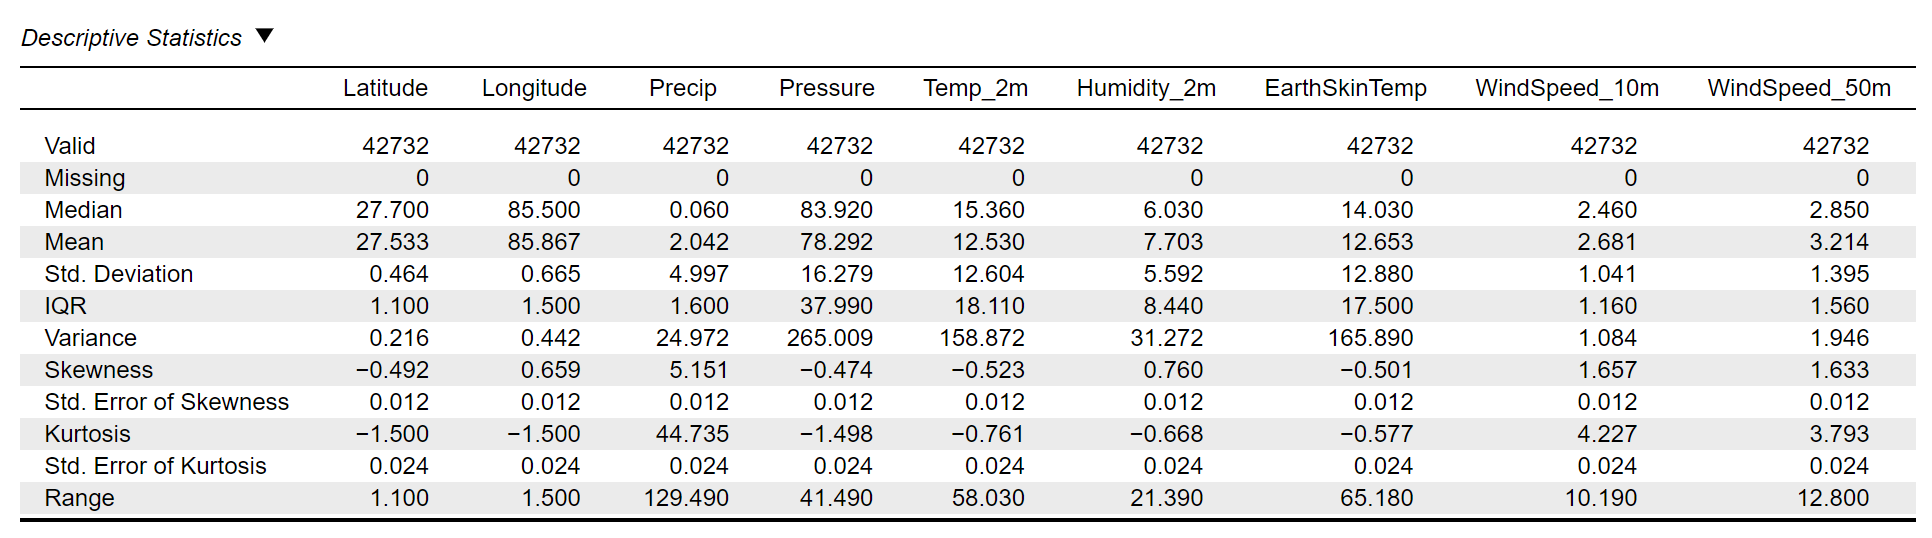
\includegraphics[width=0.7\textwidth]{figures/jasp_descriptivestats.png}
\caption{Descriptive Statistics}
\end{figure}

\textbf{Interpretation:}\\
This table presents key statistics of climate variables:

\begin{itemize}
    \item Sample size is 42,732 with no missing data.
    \item Mean temperature (12.5°C) is lower than median (15.36°C), indicating skew.
    \item Precipitation is low on average (2.04 mm) but with occasional heavy events (max 129.49 mm).
    \item Temperature and precipitation show moderate variability (SD ~12.6 and ~5.0).
    \item Negative skewness in temperature; positive skewness and higher kurtosis in precipitation and wind speed suggest occasional extremes.
\end{itemize}

To visually interpret the Descriptive Statistics, you can use the following graphical representations in JASP:

\subsection*{Histograms for distribution analysis}

Steps to generate histogram in JASP:

\begin{enumerate}
    \item Click Analyses $\rightarrow$ Descriptives $\rightarrow$ Descriptive statistics
    \item Select the variables
    \item Under Frequency Plots, check Histogram.
\end{enumerate}

\begin{figure}[h]
\centering
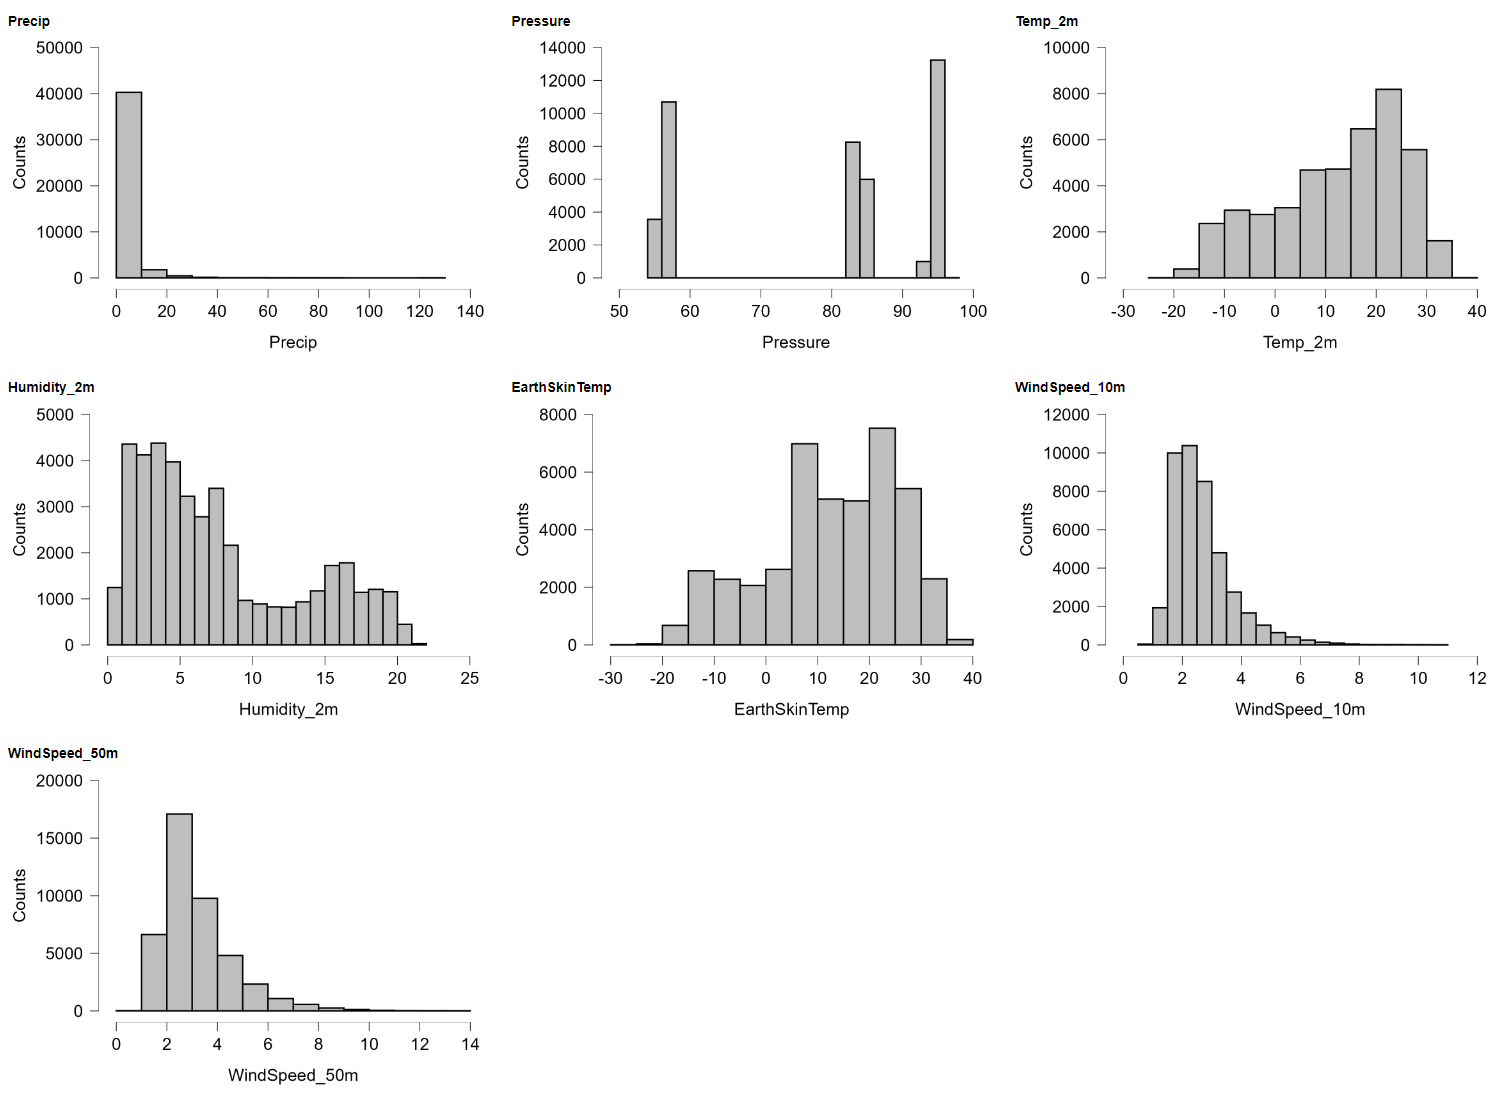
\includegraphics[width=0.7\textwidth]{figures/histogram.png}
\caption{Histogram plot}
\end{figure}

\subsection*{Boxplot}

Boxplots for outlier detection Steps to Generate Boxplots in JASP:
\begin{enumerate}
    \item Click Analyses $\rightarrow$ Descriptives $\rightarrow$ Descriptive statistics
    \item Select the variables
    \item Under Customizable Plots, check Boxplot

\end{enumerate}

\begin{figure}[h]
\centering
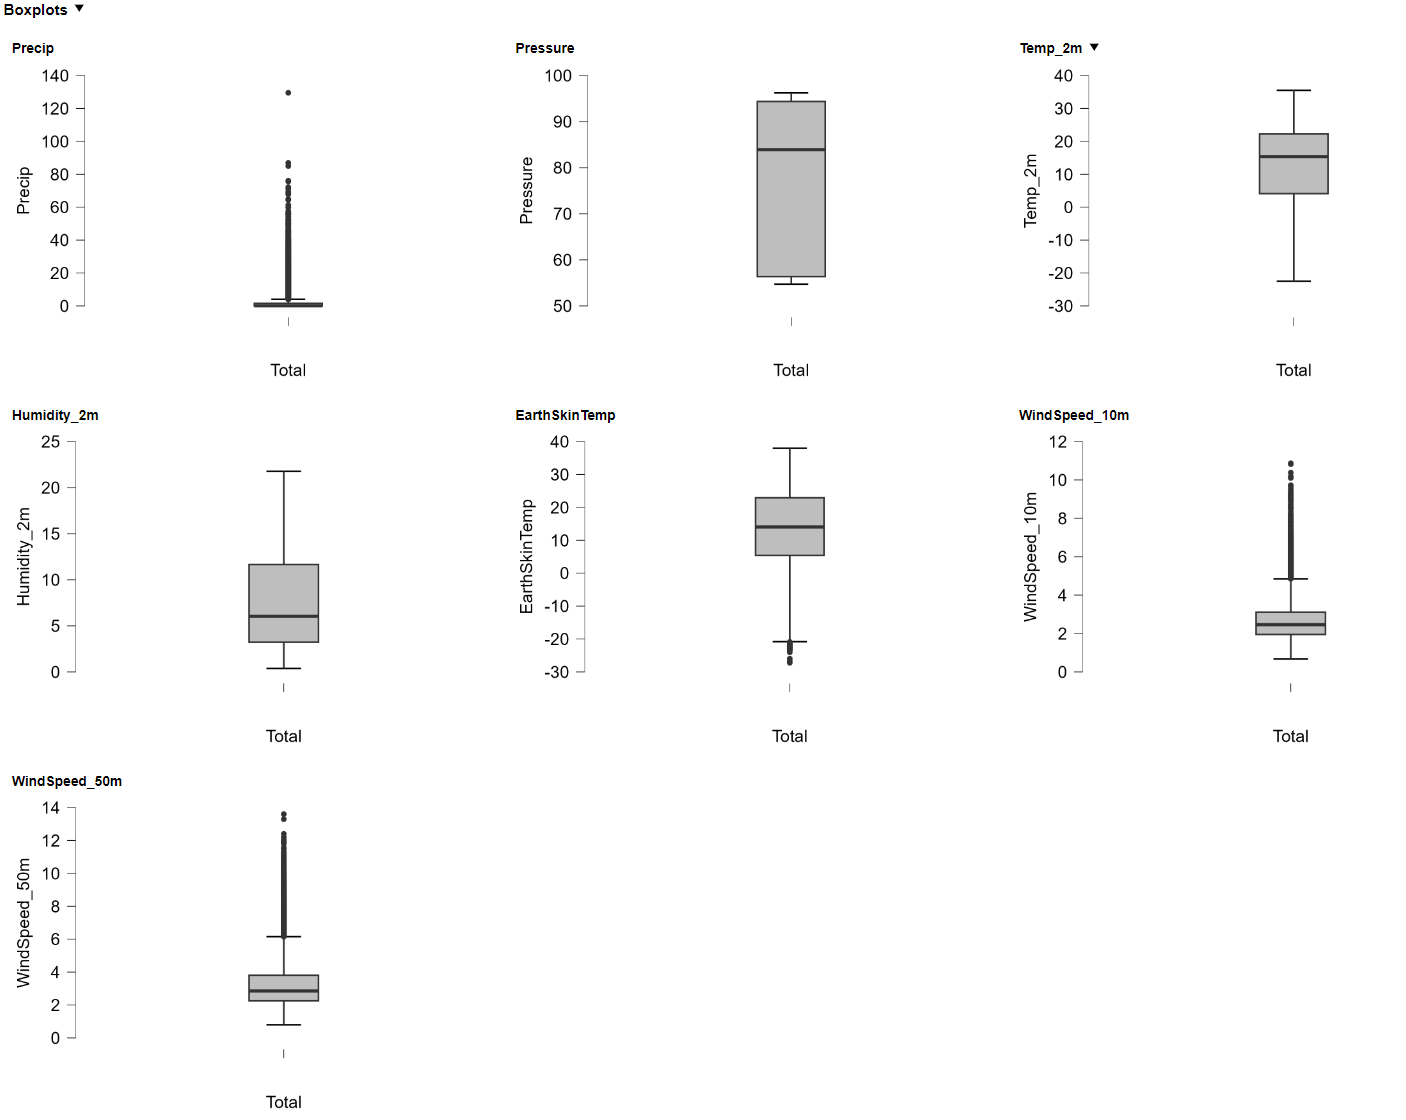
\includegraphics[width=0.7\textwidth]{figures/boxplot.png}
\caption{Boxplot}
\end{figure}

\clearpage